\documentclass[10pt,letterpaper]{article}
\usepackage{toolsper}
%\settextfont{B Nazanin}
\usepackage{lipsum}
\setlength{\parindent}{0mm}
\setlength{\parskip}{3mm}
\newcommand{\pic}[2]{
\begin{center}
\includegraphics[width=#2]{#1}
\end{center}
}
\begin{document}
\Large
\begin{center}
به نام او

پاسخ تمرینات سری نهم درس احتمال مهندسی
\hl
\end{center}
{\color{red}
نکته مهم:
$$
\int_a^b\delta(x-c)dx=\begin{cases}
1&,\quad a<c<b\\
0&,\quad \text{در غیر این صورت}
\end{cases}
$$
}

سوال 1) الف) 
$$
P=\int_0^{2\lambda}{1\over \lambda}e^{-{x\over\lambda}}dx
=\int_0^{2}e^{-x}dx=1-e^{-2}\approx0.86
$$

ب) 
$$
P=\int_{3\lambda}^{3.5\lambda}{1\over \lambda}e^{-{x\over\lambda}}dx
=\int_3^{3.5}e^{-x}dx=e^{-3}-e^{-3.5}\approx0.02
$$

سوال 2) الف)
$$
\int_{-\infty}^\infty f_X(x)dx=\int_0^16x^2(1-x)dx+\int_{-\infty}^{\infty}k\delta(x+1)dx={1\over2}+k=1
$$
پس
$
k={1\over 2}
$
.

ب)
$$
F(x)=\int_{-\infty}^xf(u)du=\begin{cases}
0&,\quad x<-1\\
{1\over 2}&,\quad -1\le x<0\\
{1\over 2}+2x^3-{3\over 2}x^4&,\quad 0\le x<1\\
1&,\quad 1\le x
\end{cases}
$$
\begin{figure}[htbp]
\centering
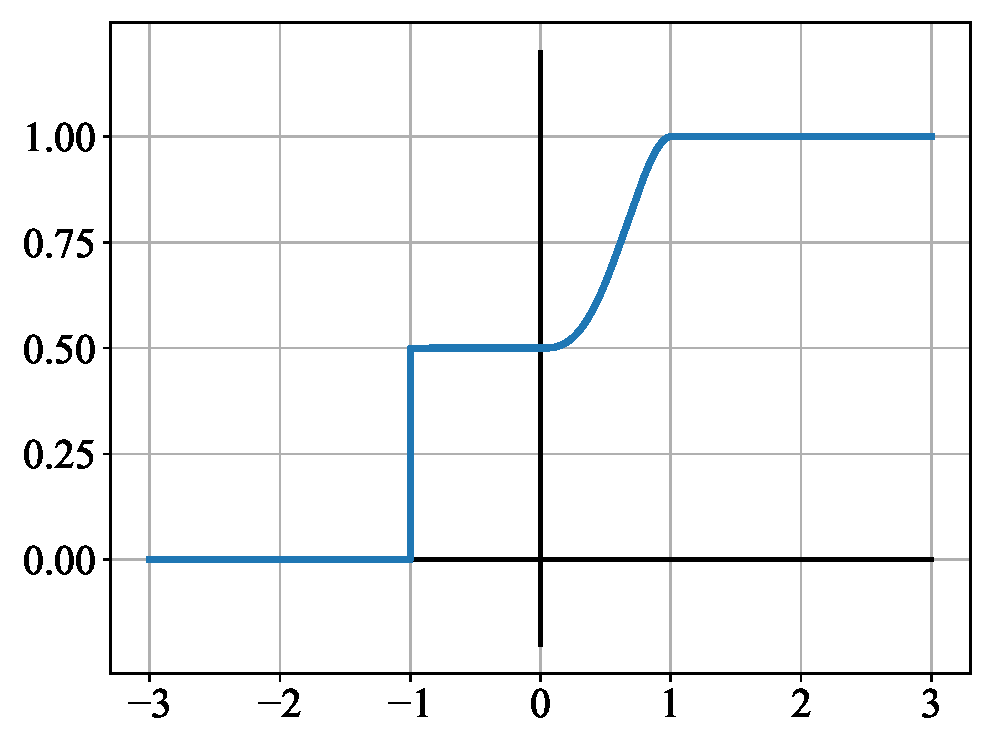
\includegraphics[width=80mm]{CDF_HW9.eps}
\end{figure}

پ)
$$
\Pr\{-2< X\le {1\over2}\}=F(0.5)-F(-2)={21\over 32}\approx0.66
$$
و
$$
\Pr\{0< X\le {1\over2}\}=F(0.5)-F(0)={5\over 32}\approx0.16
$$

سوال 3) الف) اگر $y<0$، در اینصورت مقدار 
$
\Pr\{Y\le y\}
$
همواره برابر صفر است؛ زیرا 
$
Y=X^2
$
نمی تواند منفی باشد. به ازای 
$
y\ge 0
$
:
\[
\begin{split}
\Pr\{Y\le y\}&=\Pr\{X^2\le y\}
=\Pr\{-\sqrt y\le X\le \sqrt y\}
\\&=\Pr\{0\le X\le \sqrt y\}=\begin{cases}
\sqrt y&,\quad y<1\\
1&,\quad y\ge1
\end{cases}
\end{split}
\]
در نتیجه
$$
F_Y(y)=\begin{cases}
0&,\quad y<0\\
\sqrt y&,\quad 0\le y<1\\
1&,\quad y\ge1
\end{cases}
$$
و
$$
f_Y(y)=\begin{cases}
\frac{1}{2\sqrt y}&,\quad 0<y<1\\
0&,\quad \text{سایر جاها}
\end{cases}
$$

ب)
\[
\begin{split}
&\Pr\{Y\le y\}=\Pr\{-\ln(1-X)\le y\}
=\Pr\{\ln (1-X)\ge -y\}
\\&=\Pr\{1-X\ge e^{-y}\}
=\Pr\{X\le 1-e^{-y}\}
=\begin{cases}
0&,\quad 1-e^{-y}\le0\\
1-e^{-y}&,\quad 0<1-e^{-y}<1\\
1&,\quad 1-e^{-y}\ge1
\end{cases}
\\&=\begin{cases}
0&,\quad y\le0\\
1-e^{-y}&,\quad 0<y\\
1&,\quad e^{-y}\le0 {\color{red}\text{(هرگز رخ نمی دهد)}}
\end{cases}
=\begin{cases}
0&,\quad y\le0\\
1-e^{-y}&,\quad 0<y
\end{cases}
\end{split}
\]
عبارت فوق، رابطه‌ی CDF بوده و PDF از مشتق CDF به صورت زیر به دست می آید:
$$
f_Y(y)=
\begin{cases}
0&,\quad y\le0\\
e^{-y}&,\quad 0<y
\end{cases}
$$

پ)
\[
\begin{split}
\Pr\{Y\le y\}&=\Pr\{\tan\pi(X-{1\over 2})\le y\}
=\Pr\{\pi(X-0.5)\le \tan^{-1}y\}
\\&=\Pr\{X-0.5\le {1\over \pi}\tan^{-1}y\}
=\Pr\{X\le {1\over 2}+{1\over \pi}\tan^{-1}y\}
\\&=\begin{cases}
0&,\quad {1\over 2}+{1\over \pi}\tan^{-1}y\le0\\
{1\over 2}+{1\over \pi}\tan^{-1}y&,\quad 0<{1\over 2}+{1\over \pi}\tan^{-1}y<1\\
1&,\quad {1\over 2}+{1\over \pi}\tan^{-1}y\ge1
\end{cases}
\\&=\begin{cases}
0&,\quad y\le-\infty{\color{red}\text{(هرگز رخ نمی دهد)}}\\
{1\over 2}+{1\over \pi}\tan^{-1}y&,\quad -\infty<y<\infty\\
1&,\quad y\ge\infty{\color{red}\text{(هرگز رخ نمی دهد)}}
\end{cases}
\end{split}
\]
پس
$$
F_y(y)={1\over 2}+{1\over \pi}\tan^{-1}y\quad,\quad f_Y(y)={1\over \pi}{1\over 1+y^2}
$$

سوال 4) 
$$
\Pr\{X<{2\over 3}\}=F_X({2\over 3})={2\over 3}
$$
و
$$
\Pr\{Y<{1\over \sqrt3}\}=F_X({1\over \sqrt3})={1\over 2}+{1\over\pi}\tan^{-1}{1\over\sqrt 3}={1\over 2}+{1\over\pi}\times{\pi\over 6}={2\over 3}
$$
دو مقدار احتمال با هم برابرند؛ زیرا تابعی که بین دو متغیر تصادفی برقرار است ($Y=\tan\pi(X-{1\over 2})$)، مقدار 
$
2\over 3
$
را به 
$
{1\over \sqrt 3}
$
نگاشت می دهد. از دیدگاه دیگر، ما دو برداشت متفاوت از یک احتمال را محاسبه کرده ایم.

سوال 5) الف) 
\[
\begin{split}
\Pr\{Y\le y\}&=\Pr\{|X|\le y\}
\\&=\begin{cases}
0&,\quad y<0\\
\Pr\{-y\le X\le y\}&,\quad y\ge 0
\end{cases}
\\&=\begin{cases}
0&,\quad y<0\\
\Pr\{X\le y\}-\Pr\{X<-y\}&,\quad y\ge 0
\end{cases}
\\&=\begin{cases}
0&,\quad y<0\\
F(y)-F(-y^-)&,\quad y\ge 0
\end{cases}
\end{split}
\]

ب) 
$$
\Pr\{Y=0\}=1-\Pr\{Y=1\}=\Pr\{X\le0\}=F(0)
$$
بنابراین
$$
F_Y(y)=\begin{cases}
0&,\quad y<0\\
F(0)&,\quad 0\le y<1\\
1&,\quad y\ge 1
\end{cases}
$$

پ) 
\[
\begin{split}
\Pr\{Y\le y\}&=\Pr\{X^2-2X\le y\}
\\&=\Pr\{X^2-2X+1\le y+1\}
\\&=\Pr\{(X-1)^2\le y+1\}
\\&=\begin{cases}
0&,\quad y+1<0\\
\Pr\{|X-1|\le \sqrt{y+1}\}&,\quad y+1\ge 0
\end{cases}
\\&=\begin{cases}
0&,\quad y<-1\\
\Pr\{1-\sqrt{y+1}\le X\le 1+\sqrt{y+1}\}&,\quad y\ge -1
\end{cases}
\\&=\begin{cases}
0&,\quad y<-1\\
\Pr\{X\le 1+\sqrt{y+1}\}-\Pr\{X< 1-\sqrt{y+1}\}&,\quad y\ge -1
\end{cases}
\\&=\begin{cases}
0&,\quad y<-1\\
F(1+\sqrt{y+1})-F(1-\sqrt{y+1})^-&,\quad y\ge -1
\end{cases}
\end{split}
\]
\end{document}